\chapter{Effect of exogenous cross-linking on the mechanical response of soft tissues}


\section*{Preface}
\addcontentsline{toc}{section}{Preface}%

    Exogenous cross-linking of soft collagenous tissues is a common method for biomaterial development and medical therapies. It is an important part of the fabrication process of BHVs, and significantly affects their mechanical properties. To enable improved applications through computational methods, physically realistic constitutive models are required. Yet, despite decades of research, development and clinical use, no such model exists. In this study, we develop the first rigorous full structural model (i.e. explicitly incorporating various features of the collagen fibre architecture) for exogenously cross-linked soft tissues. This was made possible, in-part, with the use of native to cross-linked matched experimental datasets and an extension to the collagenous structural constitutive model so that the uncross-linked collagen fibre responses could be mapped to the cross-linked configuration. This allowed us to separate the effects of cross-linking from kinematic changes induced in the cross-linking process, which in turn allowed the non-fibrous tissue matrix component and the interaction effects to be identified. It was determined that the matrix could be modelled as an isotropic material using a modified Yeoh model. The most novel findings of this study were that: (i) the effective collagen fibre modulus was unaffected by cross-linking and (ii) fibre-ensemble interactions played a large role in stress development, often dominating the total tissue response (depending on the stress component and loading path considered). An important utility of the present model is its ability to separate the effects of exogenous cross-linking on the fibres from changes due to the matrix. Applications of this approach include the utilization in the design of novel chemical treatments to produce specific mechanical responses and the study of fatigue damage in bioprosthetic heart valve biomaterials.

\textbf{The work contained in this chapter was published as}:  Sacks, M. S.; Zhang, W. \& Wognum, S.
A novel fibre-ensemble level constitutive model for exogenous cross-linked collagenous tissues 
Interface Focus, The Royal Society, 2016, 6, 20150090 


%---    INTRODUCTION
\section{Introduction}

    The application of exogenous-cross-links (EXLs) to native or biologically derived soft collagenous tissues finds its way into a wide range of medical therapies and device applications, such as surgical biomaterials, modification of corneal tissues (using riboflavin/UVA) and vascular grafts. Perhaps the most mechanically demanding application is the so-called bioprosthetic heart valve (BHV), which is fabricated from several types of biologically derived soft collagenous tissue membranes. From a clinical perspective, BHVs have important advantages in that they do not require permanent anticoagulation therapy, operate noiselessly, and have blood flow characteristics similar to the native valve, and thus have become the dominant heart valve therapy worldwide \cite{bini_noncollagenous_1999}\cite{schoen_cardiac_2005}\cite{schoen_founders_1999}. However, BHV durability continues to remain limited to the range of 10–15 years, resulting from leaflet structural deterioration mediated by fatigue and/or tissue mineralization \cite{vesely_tissue_2001}\cite{sacks_calcification_1999}. In general, structural damage is a critical factor in BHV degeneration, and clearly implicates coupled material and design factors as major limiters to long-term durability \cite{schoen_calcification_2005}\cite{schoen_pathology_2001}. However, a major reason why advances in the use of cross-linked tissues in BHVs and other biomedical applications is a dearth of knowledge on how EXLs affect the underlying tissue structure and macroscopic mechanical behaviour. Moreover, integration of such information into truly predictive modelling cannot proceed without accurate constitutive models of the EXL tissues and the subsequent fatigue processes \cite{sacks_incorporation_2003}\cite{sun_finite_2005}.


    The most common medical applications of cross-linked biologically-derived tissues are for dense collagenous tissues. Such tissues are typically composed of a dense, highly-organized network of type I collagen fibres, along with elastin, proteoglycans, glycosaminoglycans, cellular materials and a small amount of other fibrillar proteins. Type I collagen is the major determinant of its mechanical behaviour \cite{parry_molecular_1988}\cite{gelse_collagens_2003} and is the major tissue component affected by EXLs. At the molecular level, tropocollagen molecules are composed of a triple helix of three alpha chains \cite{parry_molecular_1988}\cite{gelse_collagens_2003} that arrange themselves into a quarter stacking array to form the collagen fibril \cite{parry_molecular_1988}\cite{gelse_collagens_2003}. Collagen fibrils form the functional subunits of the collagen fibres, as described by the Hodge–Petruska model \cite{parry_molecular_1988}\cite{petruska_subunit_1964}, and then exhibit distinct large-scale structures (figure 1). Like the fibrils from which their functional properties are derived, collagen fibres exhibit high tensile but low flexural stiffness \cite{sacks_biomechanics_2009}. We note that there is no standard definition for a fibre and its relation to the fibril. They are very dependent on the specific tissues involved, and thus caution should always be exercised in the terminology used. In the mainstream tissue biomechanics literature, the fibre/fibril definition is often taken from the well-known work of Kastelic et al. \cite{nimni_collagen_2018}, which focused on tendon. The pericardial tissues considered in this study clearly show fibre and fibril structures, including the fibre undulations commonly observed optically \cite{shen_stress_2008} (figure 1).
    
    
    The fibre longitudinal/axial direction is the primary determinant of the stiffness of the tissue composite. Interestingly, collagen fibres typically have a stiffness of 1 GPa \cite{shen_stress_2008}\cite{gentleman_mechanical_2003}\cite{eppell_nano_2006}\cite{yang_mechanical_2008} and extend by no more than 4–5\%. 
    To increase the tissue-level compliance, collagen fibres at the macroscopic scale are sinusoidally crimped \cite{parry_molecular_1988}. Tissue-level stress will not occur until the fibre-level crimp has been straightened. Moreover, the distribution of fibre straightening strains is the mechanism of tissue nonlinearity at large strains \cite{lanir_constitutive_1983}\cite{sacks_multiaxial_2003}. Thus, as in many other fields, the connection to the underlying structure can greatly inform our understanding of how collagenous tissues work and guide the development of mathematical models of their mechanical function.


    While there is a wide range of application-specific chemical agents (e.g. riboflavin/UVA cross-linking for corneas), for mechanically-demanding and blood\Hyphdash contacting applications (e.g. BHVs) using collagenous tissues, an aqueous solution of glutaraldehyde (GLUT) is used. GLUT application is necessary to both biochemically and mechanically stabilize the tissue for in vivo use. During the cross-linking process GLUT rapidly permeates the tissue, with the cross-linking process largely complete within an hour and essentially stabilized by 24 hrs. Much of what we know about how GLUT EXLs alter the structures of collagenous tissues was reported by Nimni, Cheung and co-workers \cite{cheung_mechanism_1990}\cite{nimni_chemically_1987}\cite{cheung_mechanism_1985}\cite{gendler_toxic_1984}\cite{cheung_presence_1983}\cite{cheung_mechanism_1982}\cite{cheung_mechanism_1982II}. Briefly, GLUT reacts primarily with e-amino groups of lysyl residues in proteins, with Michael-addition reaction products of Schiff bases usually the final stable products. Based on the spectral characteristics and the molecular weights of the reaction products, it has been predicted that GLUT reacts with free amines to form an intermediate with a molecular weight of about 200 Da. The GLUT–polymer amine complex is self-limiting in size and can undergo internal rearrangement to become chemically inert. An increased molecular length of GLUT polymers from the initial glutaraldehyde and lysyl-residue reaction is more likely than an increased number of cross-linked sites. Following free GLUT depletion by binding to reactive groups, additional GLUT molecules attached to already reacted molecules can give rise to larger GLUT polymers that are able to generate ‘long-range cross-links’ between further removed reactive sites (figure 2). It is apparent from a mechanical behaviour perspective that GLUT-associated chemical cross-linking of the collagen structure and biochemistry can produce complex changes from the native state at the molecular, fibril, fibre and tissue levels.
    
    
    To enable improved application of the use of EXL tissues in in situ treatment and prosthesis design, the development of physically realistic constitutive models is clearly required. In a previous work, a structural approach was used that incorporated experimentally measured angular distribution of collagen fibres and an assumed isotropic form for the EXL matrix \cite{sacks_structural_2000}. Good agreement with the experimental data was observed, supporting the basic approach. An important utility of that early model was its ability to separate the effects of the fibres and matrix. However, it was only a first step; other factors such as bending rigidity of EXL fibres, fibre–fibre interactions, and fibre–matrix interactions were not considered. Moreover, the experimental data were reduced under the assumption of an isotropic Fung model; no rigorous investigation of the most appropriate form was undertaken.
    
    
    The focus of the present work is to more fully investigate the underlying characteristics of the effects of EXLs on soft collagenous tissues, and to use this information to develop a meso-scale (i.e. at the level of the fibre) structural constitutive model. In particular, we explored the following questions of the effects of EXLs on native collagenous tissues: (i) what are the effects on individual collagen fibres, (ii) what are the effects on single collagen fibre ensembles, (iii) are there interactions between fibre ensembles, and (iv) what is the functional form of the effective matrix response? This was done by exploiting experimental data from \cite{sun_biaxial_2003}, wherein structurally controlled pericardial specimens were tested in the native state and then the EXL state. From these results, a comprehensive structural constitutive model was developed for EXL collagenous tissues and its predictive capability was evaluated. We note that, while we ultimately seek the micro-mechanical basis for macro-scale function, the present work is focused on a fibre-ensemble level approach.
    
    
    



%---    Experimental methods and data post-processing
\section{Experimental methods and data post-processing}

\subsection{Tissue sources and experimental methods} \label{c3:sec:21}

    Details of the tissue source, preparation and mechanical evaluation have been previously presented \cite{sun_biaxial_2003}. Briefly, large sections of native bovine pericardium were stored in phosphate-buffered saline (pH 7.4) at $4^\circ C$, then optically cleared using a hyperosmotic solution and the collagen fibre architecture (CFA) quantified. From the resulting CFA information, $25\times25$ mm test specimens exhibiting a high degree of structural uniformity suitable for biaxial testing were selected. The collagen fibre preferred and cross-preferred directions were aligned to the $X_1$-$X_2$ axes (figure \ref{c3:fig:3}). A total of five specimens were prepared in the native state.
    
%%%%%%%%%%%%%%%%%%%%	begin FIGURE 	%%%%%%%%%%%%%%%%%%%%
\begin{figure}
\centering
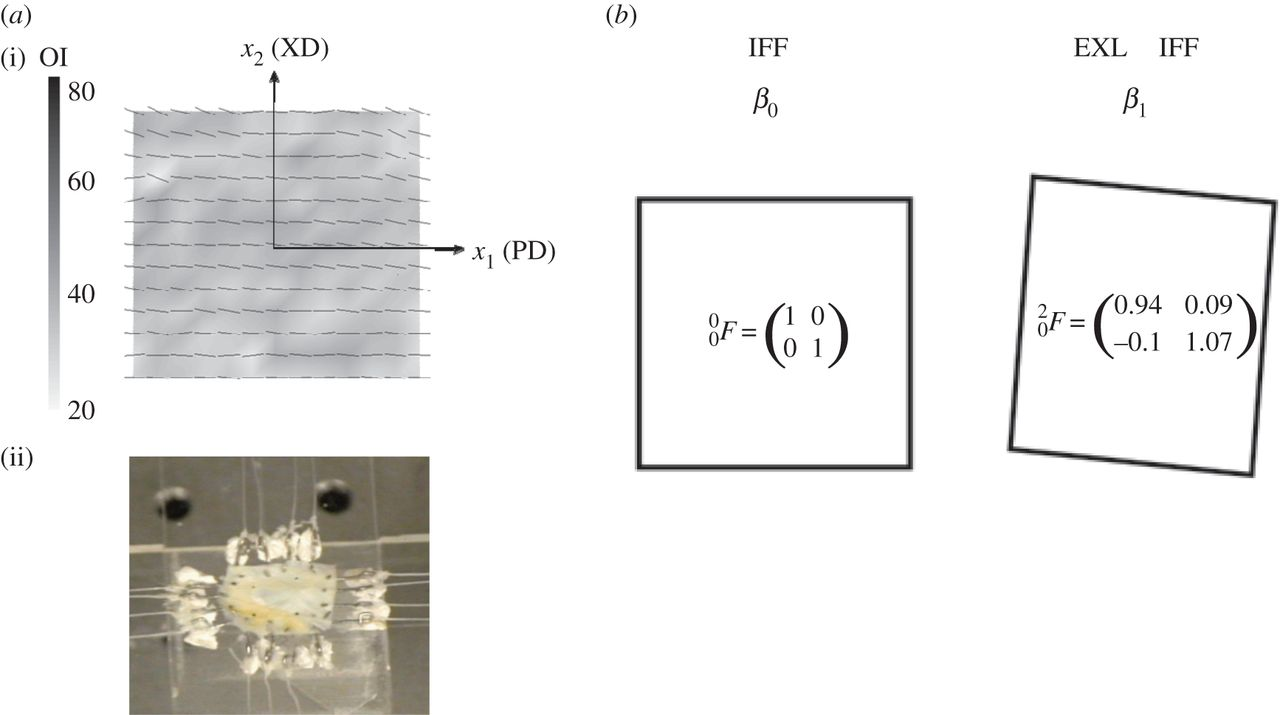
\includegraphics[width=\textwidth]{Images/chapter3/F3large.jpg}
\caption{a)(i) Pericardial test specimen showing a high degree of fibre orientation and uniformity in preferred fibre directions, with the PD = $X_1$ and XD = $X_2$ axes defined, and (ii) a typical biaxial test specimen mounted on the device. (b) A schematic of the biaxial test specimen geometry changes with cross-linking and the corresponding mean deformation gradient tensor components in native state $\beta_0$ and EXL state state $\beta_1$. Here, cross-linking induced a 6\% contraction in the PD and and 7\% direction in the XD, with some small shearing.}
\label{c3:fig:3}
\end{figure}
%%%%%%%%%%%%%%%%%%%%	 end FIGURE 	%%%%%%%%%%%%%%%%%%%%

    Biaxial mechanical testing methods have been previously described in detail \cite{sacks_orthotropic_1998,sacks_method_1999}. Briefly, testing was performed with the specimen immersed in phosphate-buffered normal saline (pH 7.4) at room temperature. First the Piola Kirchhoff stress $\mathbf{P}$ controlled test protocol was used, wherein the ratio of the normal stress components $P_{11}$:$P_{22}$ was kept constant, with $P_{12} = P_{21} = 0$ and a maximum stress level of 1 MPa was used. Tissue deformations were quantified from the motion of four markers placed in the central third of the specimen, from which the deformation gradient tensor $\mathbf{F}$ was determined. For the first testing phase, an equi-biaxial stress protocol (i.e. $P_{11}$:$P_{22}$ = 1 : 1) was used for both preconditioning and data acquisition. A total of 15 contiguous cycles were run with an approximate strain rate of 0.01 $s^{-1}$. Next, seven successive protocols were performed using ratios $P_{11}$:$P_{22}$ = 1 : 0.1, 1 : 0.5, 1 : 0.75, 1 : 1, 0.75 : 1, 0.5 : 1 and 0.1 : 1. This range was chosen for extensive coverage of in-plane strain state. After testing, each native specimen was allowed to mechanically re-equilibrate by storing them in a stress-free state at $4^\circ C$ for 24 h. Next, each specimen was chemically treated with 0.625\% GLUT for a minimum of 72 h, with the tissue marker dimensions monitored throughout the cross-linking procedure, and then stored in phosphate-buffered normal saline at $4^\circ C$. As a final step, the above biaxial testing sequence was repeated. Data post-processing included computation of the second Piola-Kirchhof tensor $\mathbf{S}$ and deformation gradient tensor $\mathbf{F}$ using established methods \cite{zhang_generalized_2015}. This test design allowed a comprehensive planar mechanical behaviour dataset to be collected on matched native and EXL specimens, compensating for inter-specimen variations.
    
    
    
    
\subsection{Kinematic considerations and mechanical data post-processing}

    As observed in our other studies \cite{sacks_biaxial_2000,zhang_generalized_2015}, the chemical fixation process will affect the specimen dimensions, and any analysis must carefully account for these effects on the collagen fibre kinematics. We thus defined the following configurations: $\beta_0$-native, $\beta_1$-EXL (figure \ref{c3:fig:3}b), used as the referential configurations for the native and EXL states, respectively. We represented all deformations using the notation for the deformation gradient tensor $\prescript{j}{i}{\mathbf{F}}$ where $i$ and $j$ represent the initial and final configurations, respectively (Nomenclature). Values for the components of $\prescript{j}{i}{\mathbf{F}}$ were determined using the same method from section \ref{c3:sec:21} for the displacements of the four markers pre- and post-cross-linking for each specimen. Next, as first described by Lanir \cite{lanir_constitutive_1983}, we defined a fibre ensemble as a group of fibres with a common orientation. It has been shown that the ensemble stress–strain relation can be obtained from the interpolated equi-biaxial strain path, where $\mathbf{F} = \operatorname{diag}[\lambda, \lambda, 1/\lambda^2]$ using $S_{ens} = S_{11} + S_{22}$ \cite{sacks_incorporation_2003}. To derive the equi-biaxial strain path $\lambda_1 = \lambda_2$ from the stress-controlled experimental data, all mechanical data were combined and interpolated using cubic Hermite patches \cite{fata_insights_2014}. A strain path with $\lambda_1 = \lambda_2$ was interpolated within the range of the data as defined by the convex hull of ($\lambda_1$, $\lambda_2$), and was implemented separately for each stress component (figure \ref{c3:fig:4}). To reliably overcome regions of sparse data we enforced the surface to be strictly convex everywhere. Finally, since the $S_{12}$ component was negligible in all specimens, it was ignored in the subsequent analyses.
    
    
%%%%%%%%%%%%%%%%%%%%	begin FIGURE 	%%%%%%%%%%%%%%%%%%%%
\begin{figure}
\centering
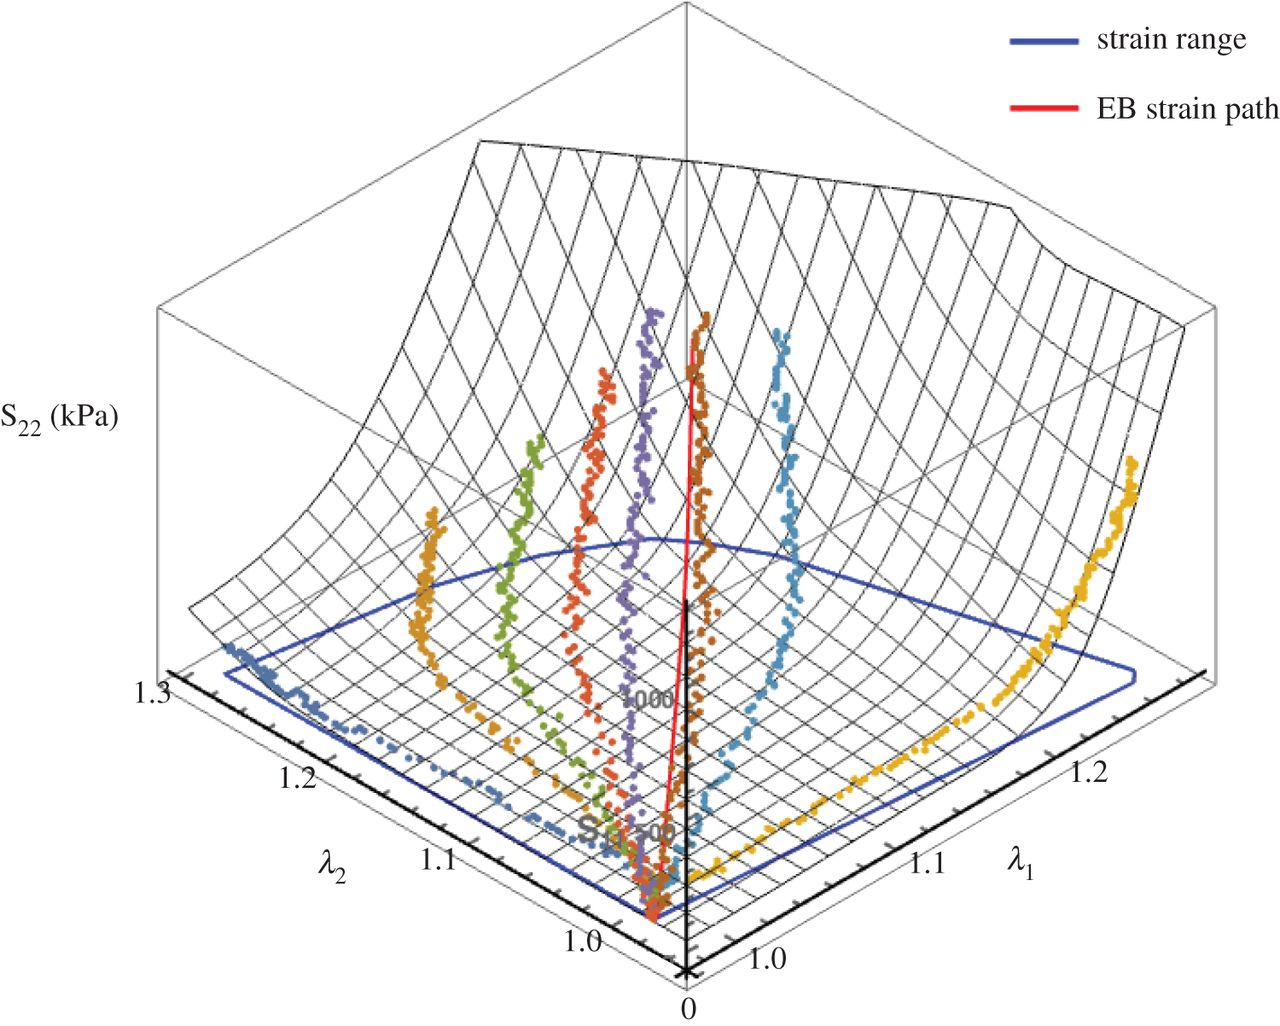
\includegraphics[width=\textwidth]{Images/chapter3/F4large.jpg}
\caption{An example of the bicubic Hermite surface interpolation of the $S_{22}$ biaxial test responses to allow interpolation of an equi-biaxial strain path, shown here in red. The blue path defines the span of the strain.}
\label{c3:fig:4}
\end{figure}
%%%%%%%%%%%%%%%%%%%%	 end FIGURE 	%%%%%%%%%%%%%%%%%%%%
    


\subsection{Establishing and modelling the mechanical behaviour of the native collagen fibre ensemble}
    
    Based on our previous tissue model findings \cite{sacks_incorporation_2003,fata_insights_2014,fan_simulation_2014,lee_presence_2015}, the dominant cause of the nonlinearity of the tissue-level mechanical behaviour of collagenous tissues is the gradual recruitment of collagen fibres \cite{lanir_constitutive_1983}. The collagen fibres themselves behave linearly under typical fibre strains experienced under physiological stresses in tissues (2–5\%). 
    Once all fibres are fully straightened, the summed response should appear linear in the ensemble response. When applied to the equi-biaxial strain derived fibre-ensemble data, the upper bound can be directly determined as the transition point between the nonlinear and linear regions, with the slope of the linear region establishing the maximum tangent modulus (MTM) of the collagen fibre ensemble (e.g. \cite{fata_insights_2014}). The matrix response can also be determined from the pre-recruitment region where no collagen fibre have contributed. To determine the recruitment upper bound in the native tissue, we started at the largest measured strain and decreased the strain level until the region above was no longer linear. Linearity was defined from the mean squared error (MSE) of the linear regression to be less than 0.005\% of the total MSE of all data, where $\mathrm{MSE} = \sum_i^n (\mathrm{S}^i_{ens} - \bar{\mathrm{S}}_{ens})/n$. Similarly, we determined the lower bound by starting at zero strain and increasing the strain until a deviation from linearity was determined.
    
    
    Next, we note that in some previous structural models a fibre stress–strain relation linear in the second Piola-Kirchhoff stress and Green Lagrange strain has been used \cite{sacks_incorporation_2003,fan_simulation_2014,lanir_structural_1979}. However, SAXS studies have demonstrated a linear force\Hyphdash displacement relation for collagen fibrils in the tendon \cite{sasaki_elongation_1996,sasaki_stress_1996} and MV tissue \cite{liao_relation_2007}. This is further corroborated by the atomistic modelling results by Buehler \cite{buehler_atomistic_2006}, where the force\Hyphdash displacement relation is essentially linear at strains lower than 0.35. We have recently determined that for the mitral valve leaflet the tissue level-derived collagen fibre mechanical behaviour is actually quite linear, with an effective modulus of approximately 160 MPa. Based on these considerations, we assumed for the native collagen fibres that
        \begin{enumerate}
            \item they exhibit a linear $P-\lambda$ response
            \item slack stretch of the collagen fibres does not vary with orientation.
        \end{enumerate}
    From these two basic considerations, we used the following effective native collagen fibre model \cite{fata_insights_2014,fan_simulation_2014}. We start by defining the native collagen fibre strain energy as
        %-------------------	begin EQUATION 	-------------------%
        \begin{equation}\label{c3:eqn:21}
        \begin{aligned}
        \Psi_f(\lambda_t) = 
            \begin{cases} 
                \frac{\eta_c}{2} \left(\lambda_t -1\right)^2 & \text{for } \lambda_t >1\\
                0 & \text{for } \lambda_t < 1  
            \end{cases}
        \end{aligned}
        \end{equation}
        %-------------------	 end EQUATION 	-------------------%
    where $\lambda_t = \lambda_f/\lambda_s$ is the true stretch of the fibre. This leads to the following $P-\lambda$ form using $P_f = \partial \Psi_f(\lambda_t)/\partial \lambda_f = \partial \Psi_f(\lambda_t)/\partial \lambda_t \cdot \partial \lambda_t/\partial \lambda_f$
        %-------------------	begin EQUATION 	-------------------%
        \begin{equation}\label{c3:eqn:22}
        \begin{aligned}
        P_f = 
            \begin{cases} 
                \frac{\eta_c}{\lambda_s} \left(\lambda_t -1\right) & \text{for } \lambda_t >1\\
                0 & \text{for } \lambda_t < 1  
            \end{cases}
        \end{aligned}
        \end{equation}
        %-------------------	 end EQUATION 	-------------------%
    where $P_f$ is the first Piola-Kirchhoff stress of the fibre, $\eta_c$ is the modulus of the fibre, $\lambda_f$ is the fibre stretch and $\lambda_s$ is the fibre slack stretch. Next, we use this fibre model in the expression for the native collagen fibre ensemble using
        %-------------------	begin EQUATION 	-------------------%
        \begin{equation}\label{c3:eqn:23}
        \begin{aligned}
        P_c^{ens} =& \phi_c\eta_c\int_1^{\lambda_\theta}\frac{D(x)}{x} \left(\frac{\lambda_\theta}{x} - 1\right) \dif x    \\
        \text{and} \quad \dpd{P_c^{ens}}{\lambda_\theta} =&\mathrm{TM}_c^{ens} = \phi_c\eta_c\int_1^{\lambda_\theta}\frac{D(x)}{x^2}\dif x,
        \end{aligned}
        \end{equation}
        %-------------------	 end EQUATION 	-------------------%
    where $\phi_c$ is the collagen fibre mass fraction, $\lambda_\theta$ is the fibre-ensemble stretch along the direction defined by $\theta$ (computed from the tissue-level deformation using $\lambda_\theta = \mathbf{F}\cdot\mathbf{n}(\theta)$), and $D(\lambda_s)$ is the probability distribution function describing the distribution of collagen fibre slack length within the ensemble. We assumed $D(\lambda_s)$ is Beta distributed, so that
        %-------------------	begin EQUATION 	-------------------%
        \begin{equation}\label{c3:eqn:24}
        \begin{aligned}
        D(\alpha, \beta, \lambda_{lb}, \lambda_{ub}, \lambda_s) =& 
            \begin{cases}
            \frac{y^{\alpha-1}(1-y)^{\beta-1}}{B(\alpha,\beta)(\lambda_{ub}-\lambda_{lb})} & \text{for } y \in [0,1] \\
            0 & \text{otherwise}
            \end{cases} \\
        y=&\frac{\lambda_s-\lambda_{lb}}{\lambda_{ub}- \lambda_{lb}}, \quad \bar{\mu} =\frac{\mu - \lambda_{lb}}{\lambda_{ub}-\lambda_{lb}}   \\
        and \quad \bar{\sigma} =& \frac{\sigma}{\lambda_{ub} - \lambda_{lb}}, \quad \alpha = \frac{\bar{\mu}^2 - \bar{\mu}^3 - \bar{\sigma}^2\bar{\mu}}{\bar{\sigma}^2},   \\
        \beta =& \alpha \frac{1-\bar{\mu}}{\bar{\mu}}
        \end{aligned}
        \end{equation}
        %-------------------	 end EQUATION 	-------------------%
    where $\lambda_{lb}$ and $\lambda_{ub}$ are the lower and upper bound stretch of the collagen fibre recruitment, respectively. Note that in preliminary examinations of the data we found that all specimens exhibited distinct pre- and post-transition locations (figure \ref{c3:fig:5}), allowing $\lambda_{lb}$ and $\lambda_{ub}$ to be determined directly from the collagen fibre ensemble data. Thus, the complete initial ensemble model (equation \ref{c3:eqn:23}) has three parameters $\{\eta_c, \alpha, \beta\}$ to fit to the data using standard techniques \cite{fata_insights_2014}.
    
    
    
    
    
%%%%%%%%%%%%%%%%%%%%	begin FIGURE 	%%%%%%%%%%%%%%%%%%%%
\begin{figure}
\centering
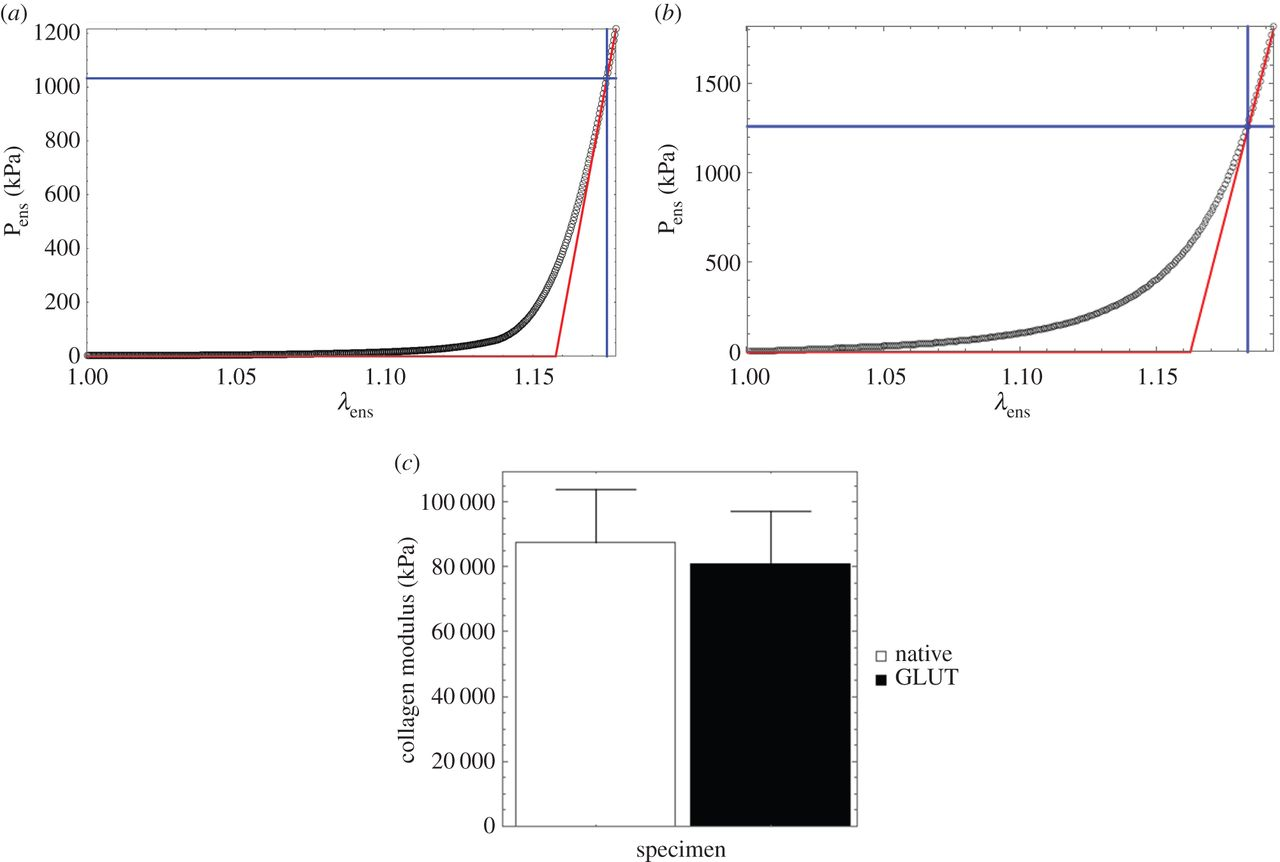
\includegraphics[width=\textwidth]{Images/chapter3/F5large.jpg}
\caption{A representative fibre-ensemble stress–strain (in $P_\mathrm{ens}-\lambda_\mathrm{ens}$) response for (a) native and (b) cross-linked bovine pericardium illustrating a well-defined post-transition fibre recruitment point wherein the response becomes linear. While the native pericardium demonstrated a very low initial modulus (approx. 75 kPa; table \ref{c3:tab:2}), the EXLs demonstrate a significantly stiffer modulus.}
\label{c3:fig:5}
\end{figure}
%%%%%%%%%%%%%%%%%%%%	 end FIGURE 	%%%%%%%%%%%%%%%%%%%%

%---    Delineation and modelling of the tissue-level mechanical effects of exogenous cross-links
\section{Delineation and modelling of the tissue-level mechanical effects of exogenous cross-links} \label{c3:sec:3}

\subsection{Rationale}

    While extensive work has been done on the characterization of the biomechanical effects of EXL formation on soft tissues \cite{sun_biaxial_2003,sacks_bioprosthetic_2006,sun_simulated_2005,sellaro_effects_2007,alferiev_prevention_2003,wells_cyclic_2005,wells_effects_2002,wells_effects_2000,wells_thermomechanical_1998,lee_high_1994,naimark_correlation_1992,lee_effect_2001,barber_mechanics_1999,mirnajafi_effects_2005}, there has been surprisingly little work done known to the authors on the development of formal constitutive models (other than \cite{sacks_structural_2000}). Related work on proteoglycan and related collagen fibril sub\Hyphdash forms have revealed complex micromechanical interactions (e.g. \cite{cavalcante_mechanical_2005,coughlin_dynamic_1996}), but micromechanical interactions modified by EXLs on the macroscale tissue responses remain largely unknown. Thus, prior to developing the constitutive model form, we first carefully examined the effects of EXL formation on the measured tissue\Hyphdash level biomechanical behaviours in the present data set.


\begin{table}
\centering
\caption{Equibiaxial strain testing results.}\label{c3:tab:2}
\begin{tabular}{L{.5in}R{.48in}R{.48in}R{.48in}R{.48in}R{.48in}R{.48in}R{.48in}R{.48in}}
\hline
\multicolumn{1}{l}{\textbf{ID}} &
\multicolumn{1}{c}{\textbf{12}} &
\multicolumn{1}{c}{\textbf{21}} &
\multicolumn{1}{c}{\textbf{41}} &
\multicolumn{1}{c}{\textbf{61}} &
\multicolumn{1}{c}{\textbf{68}} &
\multicolumn{1}{c}{\textbf{mean}} &
\multicolumn{1}{c}{\textbf{s.e.m.}} &
\multicolumn{1}{c}{\textbf{p-value}}\\
\hline
\multicolumn{9}{c}{initial tangent modulus (kPa)} \\
\hline
native & 73.9 & 65.6 & 25.5 & 110.6 & 107.3 & 76.6 & 17.4 & \\
\hline
GLUT & 1059.3 & 248.4 & 152.4 & 746.0 & 272.1 & 495.6 & 195.2 & 0.037   \\
\hline
\multicolumn{9}{c}{MTM (kPa)} \\
\hline
native & 54208 & 49014 & 53091 & 72460 & 77121 & 61179 & 6341.3 &   \\
\hline
GLUT & 67771 & 28615 & 58025 & 62319 & 70718 & 57490 & 8433.8 & 0.567 \\
\hline
\multicolumn{9}{c}{upper bound stress (kPa)} \\
\hline
native & 1164.0 & 885.4 & 956.2 & 1048.4 & 1289.4 & 1068.7 & 80.80 &  \\
\hline
GLUT & 1081.7 & 925.8 & 1204.2 & 1138.2 & 1353.8 & 1140.8 & 78.69 & 0.245   \\
\hline
\end{tabular}
\end{table}





\subsection{Effects of exogenous cross-link formation on collagen fibre ensembles}

    All specimens exhibited anisotropic dimensional changes due to preconditioning and cross-linking (figure \ref{c3:fig:3}b). Interestingly, we found that about 6\% shrinkage occurred in the preferred direction, and approximately 7\% expansion in the cross-preferred directions. Such changes can alter both the angular dependence on collagen recruitment and the collagen fibre orientation distribution. We determined basic characteristics of the collagen fibre stress–strain relations directly from the data (no modelling), including the lower and upper bound-associated stresses, the initial tangent modulus, and the MTM from a running 15-point window. From this analysis, we were able to determine a number of important mechanical characteristics (table 2 and figure \ref{c3:fig:5}). These include:
        \begin{enumerate}
            \item All specimens exhibited an approximately 6.5-fold increase in the initial tangent modulus (table 2), very similar to values and native/EXL ratios reported in \cite{mirnajafi_effects_2005}, which were conducted under flex conditions.
            \item The upper bound stress and MTM were found to be unaffected by EXL formation (table 2).
            \item EXL formation induced a reduction in achieved strain levels compared with the native state (figure \ref{c3:fig:5}a).
            \item The effective collagen modulus was unaffected by EXL formation (figure \ref{c3:fig:5}c).
        \end{enumerate}
    Collectively, these results reveal some important features of the effects of EXLs on collagen tissues. First, as noted in our previous studies \cite{sacks_structural_2000,mirnajafi_effects_2005} EXLs produce a substantial increase in the low-strain modulus. Next, equation \ref{c3:eqn:23} indicates that the MTM is proportional to the collagen fibre modulus and the recruitment function D. Use of equation \ref{c3:eqn:23} compensates for the effect of the changes in tissue dimensions due to cross-linking on the fibre recruitment, allowing separation of changes in fibre architecture from the modulus on the ensemble stress–strain curve. Thus, the lack of changes in effective modulus are independent of any effects of changes resulting from tissue dimensions and represent an accurate modulus estimate.
    
    
    

%---    Initial model formulation
\section{Initial model formulation}

\subsection{General approach}

    The above findings provide sufficient information to develop a new model. In the present study, we assume EXLs induce fibre–fibre and fibre–matrix interactions that are mechanically significant. We ignore any time-dependent effects, as we have found that native and cross-linked valvular tissues exhibit minimal time-dependent effects \cite{grashow_planar_2006,grashow_biaxial_2006,stella_time_2007,eckert_biomechanical_2013}. Next, we assume that the pericardial tissues considered are only composed of collagen fibres and a matrix constituent that represents non-cross-linked and cross-linked components, and water. The contributions from elastin or other tissue components are ignored, because they have either negligible mass or stiffness. In all previous structural models of soft tissues, interactions between components (fibres, matrix) have been ignored. As we cannot assume this in the present investigation, we use the following hyperelastic general form:
        %-------------------	begin EQUATION 	-------------------%
        \begin{equation}\label{c3:eqn:41}
        \begin{aligned}
        \Psi(\mathbf{C}) = \phi_c[\Psi_c(\mathbf{C} +\Psi_\mathrm{int}(\mathbf{C}] + (1-\phi_c)\Psi_m(\mathbf{C} + p(J-1)
        \end{aligned}
        \end{equation}
        %-------------------	 end EQUATION 	-------------------%
    where $\phi_c$ is the mass fraction of the collagen fibres, $\phi_c$, $\phi_m$ and $\phi_\mathrm{int}$ are the strain energy density functions of the collagen, matrix and interaction terms, respectively, $J=\operatorname{det}(\mathbf{F})$, and $p$ is the Lagrange multiplier to enforce incompressibility. The resulting tissue-level response in terms of the second Piola-Kirchhoff stress tensor $\mathbf{S}$ is given by
        %-------------------	begin EQUATION 	-------------------%
        \begin{equation}\label{c3:eqn:42}
        \begin{aligned}
        \mathbf{S} =& 2\dpd{\psi}{\mathbf{C}} - p\mathbf{C}^{-1} \\
            =& 2\left[\phi_c\dpd{\Psi_c}{\mathbf{C}} + (1-\phi_c) \dpd{\Psi_m}{\mathbf{C}} + \phi_c \dpd{\Psi_\mathrm{int}}{\mathbf{C}}\right] - p\mathbf{C}^{-1}.
        \end{aligned}
        \end{equation}
        %-------------------	 end EQUATION 	-------------------%
        



\subsection{Accounting for changes in tissue dimensions for the collagen phase} \label{c3:sec:42}

    Results from section \ref{c3:sec:3} suggest that the native collagen fibre modulus is unaffected by cross-linking. However, the observed changes in tissue dimensions can also induce changes in tissue-level mechanical behaviour by altering the structure due to tissue shrinkage. This essentially results in a different reference configuration. There is thus a need to reformulate structural models to account for these effects directly. The formulation described in the following allows handling of changes in tissue reference state geometry. The key assumptions are:
        \begin{enumerate}
            \item Changes are due to alterations in the initial geometric configuration only, so that
            \begin{enumerate}
                \item Mass fractions of each phase remain unchanged.
                \item The internal mechanical energy remains zero. Thus, all changes in internal component configurations are not associated with any change in internal energy (which remains zero)—just initial configuration (e.g. fibre orientation, degree of undulation, thickness and length).
            \end{enumerate}
            \item Tissue dimensions and internal architecture change under the \textit{affine} kinematic assumption. Thus, the configuration of all constituent fibres in the altered reference state (after all changes in initial specimen geometry have taken place) can be predicted. Moreover, the configurational change is homogeneous, and can be thus described by a deformation gradient tensor with constant components.
            \item To be consistent with the fibre recruitment mechanisms (e.g. \cite{sacks_incorporation_2003,fata_insights_2014}), all fibres remain undulated in the new reference state.
            \item The matrix phase is unaffected by the geometric configuration changes and is referenced to $\beta_1$ (figure \ref{c3:fig:3}b) for all subsequent stress calculations.
        \end{enumerate}
        
        
    As a first step, we recast the recruitment function parameters determined in $\beta_0$ but mapped to $\beta_1$ using
        %-------------------	begin EQUATION 	-------------------%
        \begin{equation}\label{c3:eqn:43}
        \begin{aligned}
        &D_1(\mu_0, \sigma_0, \prescript{}{0}{\lambda}_{lb}, \prescript{}{0}{\lambda}_{ub}, \prescript{1}{0}{\lambda}, \prescript{}{1}{\lambda}_s) = 
            \begin{cases}
            \frac{y^{\alpha-1}(1-y)^{\beta-1}}{B(\alpha,\beta)(\prescript{}{1}{\lambda}_{ub}-\prescript{}{1}{\lambda}_{lb})} & \text{for } y \in [0,1] \\
            0 & \text{otherwise}
            \end{cases} \\
        &y=\frac{\prescript{t}{1}{\lambda}_s-\prescript{}{1}{\lambda}_{lb}}{\prescript{}{1}{\lambda}_{ub}- \prescript{}{1}{\lambda}_{lb}}, 
        \quad \prescript{}{1}{\lambda}_{ub} = \frac{\prescript{}{0}{\lambda}_{ub}}{\prescript{1}{0}{\lambda}}, 
        \quad \prescript{}{1}{\lambda}_{lb} = \frac{\prescript{}{0}{\lambda}_{lb}}{\prescript{1}{0}{\lambda}}   \\
        &\bar{\mu} =\frac{\mu - \prescript{}{0}{\lambda}_{lb}}{\prescript{}{0}{\lambda}_{ub}-\prescript{}{0}{\lambda}_{lb}},
        \quad \bar{\sigma} = \frac{\sigma}{\prescript{}{0}{\lambda}_{ub} - \prescript{}{0}{\lambda}_{lb}}, \\
        &\alpha = \frac{\bar{\mu}^2 - \bar{\mu}^3 - \bar{\sigma}^2\bar{\mu}}{\bar{\sigma}^2},  
        \quad \beta = \alpha \frac{1-\bar{\mu}}{\bar{\mu}}
        \end{aligned}
        \end{equation}
        %-------------------	 end EQUATION 	-------------------%
    where the left subscript denotes the configuration state. Note carefully that $\prescript{1}{0}{\lambda}$ will in general be a function of $\theta_1$, so that even though the collagen fibre recruitment is orientation-independent in $\beta_0$, it will have angular dependence in $\beta_1$ unless $\prescript{1}{0}{F}_{11} = \prescript{1}{0}{F}_{22}$ and $\prescript{1}{0}{F}_{12} = \prescript{1}{0}{F}_{21} = 0$. The resulting expression for the ensemble stress is
        %-------------------	begin EQUATION 	-------------------%
        \begin{equation}\label{c3:eqn:44}
        \begin{aligned}
        \prescript{t}{1}{\mathbf{S}}_c^{ens} = \phi_c\frac{\eta_c}{\prescript{t}{1}{\lambda}}
            \int_1^{\prescript{t}{1}{\lambda}} \frac{D_1(x)}{x}\left(\frac{\prescript{t}{1}{\lambda}}{x} - 1\right) \dif x
        \end{aligned}
        \end{equation}
        %-------------------	 end EQUATION 	-------------------%
    To complete the tissue-level formulation, we use the affine transformation assumption and the formulation described in \cite{fan_simulation_2014} to obtain the collagen fibre orientation distribution function $\Gamma_0$ in the native state to that in $\beta_1$ using
        %-------------------	begin EQUATION 	-------------------%
        \begin{equation}\label{c3:eqn:45}
        \begin{aligned}
        \Gamma_1[\mu_\Gamma,\sigma_\Gamma, \theta_1 = \Gamma_0[\mu_\Gamma, \sigma_\Gamma, \theta_0(\prescript{1}{0}{\mathbf{F}},\theta_1)\frac{\prescript{1}{0}{\lambda}_{\theta_0}^2}{\prescript{1}{0}{J_\mathrm{2D}}}].
        \end{aligned}
        \end{equation}
        %-------------------	 end EQUATION 	-------------------%
    Note that the angle $\theta_1$ of a fibre originally oriented at $\theta_0$ can be determined using
        %-------------------	begin EQUATION 	-------------------%
        \begin{equation}\label{c3:eqn:46}
        \begin{aligned}
        \theta_1(\prescript{1}{0}{\mathbf{F}},\theta_0) = \tan^{-1}\left(\frac{\prescript{1}{0}{F}_{21}\cos{\theta_0} + \prescript{1}{0}{F}_{22}\sin{\theta_0}}{\prescript{1}{0}{F}_{11}\cos{\theta_0} + \prescript{1}{0}{F}_{12}\sin{\theta_0}}\right)
        \end{aligned}
        \end{equation}
        %-------------------	 end EQUATION 	-------------------%
    The final form of the native collagen fibre phase expressed in the EXL state is thus
        %-------------------	begin EQUATION 	-------------------%
        \begin{equation}\label{c3:eqn:47}
        \begin{aligned}
        \prescript{t}{1}{\mathbf{S}}(\eta_c, \mu_\Gamma, \sigma_\Gamma, \mu_0, \sigma_0)& = \phi_c\frac{\eta_c}{\prescript{t}{1}{\lambda}} \int_{\theta_1} \Gamma_1(\mu_\Gamma, \sigma_\Gamma,\theta_1))
        \\
        &\left\{ \frac{D_1(\mu_0, \sigma_0, \prescript{}{0}{\lambda}_{lb}, \prescript{}{0}{\lambda}_{ub},\prescript{1}{0}{\lambda}[\theta_0(\theta_1)],x)}{x}\left(\frac{\prescript{1}{0}{\lambda}}{x} - 1\right)\dif x\right\}\mathbf{n}_1\otimes\mathbf{n}_1 \dif \theta
        \end{aligned}
        \end{equation}
        %-------------------	 end EQUATION 	-------------------%
    The above equation has a total of five fitted model parameters $\eta_c$, $\mu_\Gamma$, $\sigma_\Gamma$, $\mu_0$, and $\sigma_0$ ($\lambda_{lb}$ and $\lambda_{lb}$ are determined from the experimental data), all with a physical meaning and all referenced to $\beta_0$.

        
\subsection{The matrix phase}

    The matrix response can be estimated from the low stress region where collagen does not contribute any stress (figures \ref{c3:fig:5} and \ref{c3:fig:6}). A careful examination revealed that the toe region is a convex curve in $S-\lambda$, which is inconsistent with a neo-Hookean material model which is concave in $S-\lambda$ (figure \ref{c3:fig:6}). While we have used an exponential isotropic function for the matrix before \cite{sacks_structural_2000}, we considered the Yeoh model but found it unable to fit the data. Therefore, we developed a modified Yeoh model as
        %-------------------	begin EQUATION 	-------------------%
        \begin{equation}\label{c3:eqn:48}
        \begin{aligned}
        \Psi_m(\mathbf{C}) =& \frac{1}{2}\frac{\mu_a}{a}(I_1 - 3)^a + \frac{1}{2}\frac{\mu_b}{b}(I_1 - 3)^b  \\
        \mathbf{S}_m =& \left(\mu_a(I_1 - 3)^{a-1} + \mu_b(I_1 - 3)^{b-1}\right)(\mathbf{I} - C_{33}\mathbf{C}^{-1}), \\
        &\quad\quad \text{with } 1<a<b, \quad a\times b < 2
        \end{aligned}
        \end{equation}
        %-------------------	 end EQUATION 	-------------------%
    When applied to all pre-transition mechanical data (i.e. from all protocols and where there is no collagen fibre contribution), this form was found to fit the low-stress data quite well (figure \ref{c3:fig:6}).
    

%%%%%%%%%%%%%%%%%%%%	begin FIGURE 	%%%%%%%%%%%%%%%%%%%%
\begin{figure}
\centering
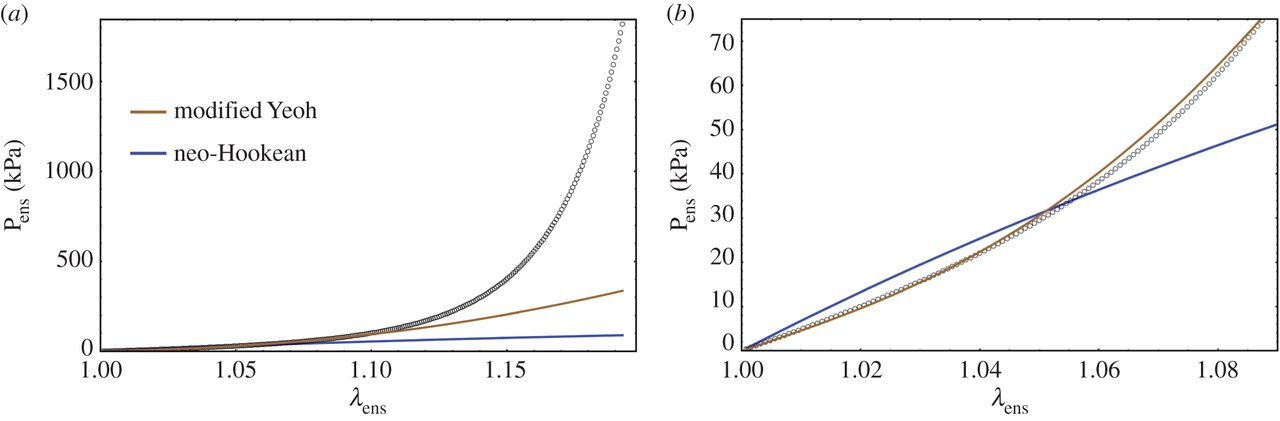
\includegraphics[width=\textwidth]{Images/chapter3/F6large.jpg}
\caption{A representative fibre-ensemble stress–strain (in $P_\mathrm{ens}-\lambda_\mathrm{ens}$)  for EXL treated bovine periardium, and (b) a close-up of the low stress region. A careful examination revealed that the toe region suggests that a modified Yeoh model was necessary to accurately capture its response (equation \ref{c3:eqn:48}) due to the convexity of the response.}
\label{c3:fig:6}
\end{figure}
%%%%%%%%%%%%%%%%%%%%	 end FIGURE 	%%%%%%%%%%%%%%%%%%%%
    
    
\subsection{Interactions}
        
    Our key working assumption is that all fibre–fibre and fibre–matrix interactions can be represented at the fibre-ensemble level. This is done to simplify the model formulation, and further since the exact micromechanical mechanisms of cross-linking have yet to be determined. Based on the form assumed in equation \ref{c3:sec:42}, we now have the ability to estimate the form and magnitude of the fibre-ensemble interactions from the fibre-ensemble data using $\mathbf{S}_\mathrm{int} \approx \mathbf{S}_\mathrm{ens} - 1/\phi_c(\phi_c \mathbf{S}_c + (1 - \phi_c)\mathbf{S}_m)$, where $\mathbf{S}_\mathrm{ens}$ is the ensemble stress (figure \ref{c3:fig:5}). Note here that the collagen stress Embedded Image and is thus the contribution of the collagen fibres expressed in the EXL configuration $\beta_1$ using equation \ref{c3:eqn:47}. This approach allowed us to exploit the matched native–EXL mechanical data by fitting the native responses then mapping them to the EXL state, so that they are a known quantity rather than one that required data fitting. Results of this analysis indicated some intriguing results. First, while the collagen phase contributed substantially to the total ensemble stress, it was only about 50\%, and the matrix only about 20\%. This revealed that the remaining approximately 30\% portion of the total ensemble stress must be a result of the interaction mechanisms.
    
    
    To model the interactions, we first consider two fibre ensembles with orientation vectors $\mathbf{n}_0(\alpha)$ and $\mathbf{m}_0(\beta)$ in the reference configuration (figure \ref{c3:fig:7}). These two ensembles can mechanically interact by elongation and relative rotation. Kinematically, these mechanisms can be captured using the pseudo-invariant $I_8$ \cite{holzapfel_nonlinear_2000,merodio_influence_2006} 
        %-------------------	begin EQUATION 	-------------------%
        \begin{equation}\label{c3:eqn:49}
        \begin{aligned}
        I_8 &= \mathbf{n}_0\cdot\mathbf{C}\mathbf{m}_0 = \cos(\theta)\lambda_\alpha\lambda_\beta \\
        \cos(\theta) &= \frac{\mathbf{n}_0\cdot\mathbf{m}_0}{\lambda_\alpha\lambda_\beta}, \quad \lambda_\alpha=\sqrt{\mathbf{n}_0\cdot\mathbf{C}\mathbf{n}_0}, \quad \lambda_\alpha=\sqrt{\mathbf{m}_0\cdot\mathbf{C}\mathbf{m}_0} 
        \end{aligned}
        \end{equation}
        %-------------------	 end EQUATION 	-------------------%
    Note that we can also use $I_8^\prime = I_8  - I_8^0$ \cite{merodio_influence_2006} to account for the relative change in fibre rotations if necessary. Thus, $i_8$ can be considered the product of an extensional term $\lambda_\alpha \lambda_\beta$ and a rotational term $\cos(\theta)$. We consider two sub-aspects of ensemble-level effects: intra- and inter-ensemble levels. The intra-ensemble incorporates all fibre–fibre interactions that occur within a single ensemble and are limited to extensional effects only. By contrast, inter-ensemble effects can include both extensional and rotational effects.
    
    
%%%%%%%%%%%%%%%%%%%%	begin FIGURE 	%%%%%%%%%%%%%%%%%%%%
\begin{figure}
\centering
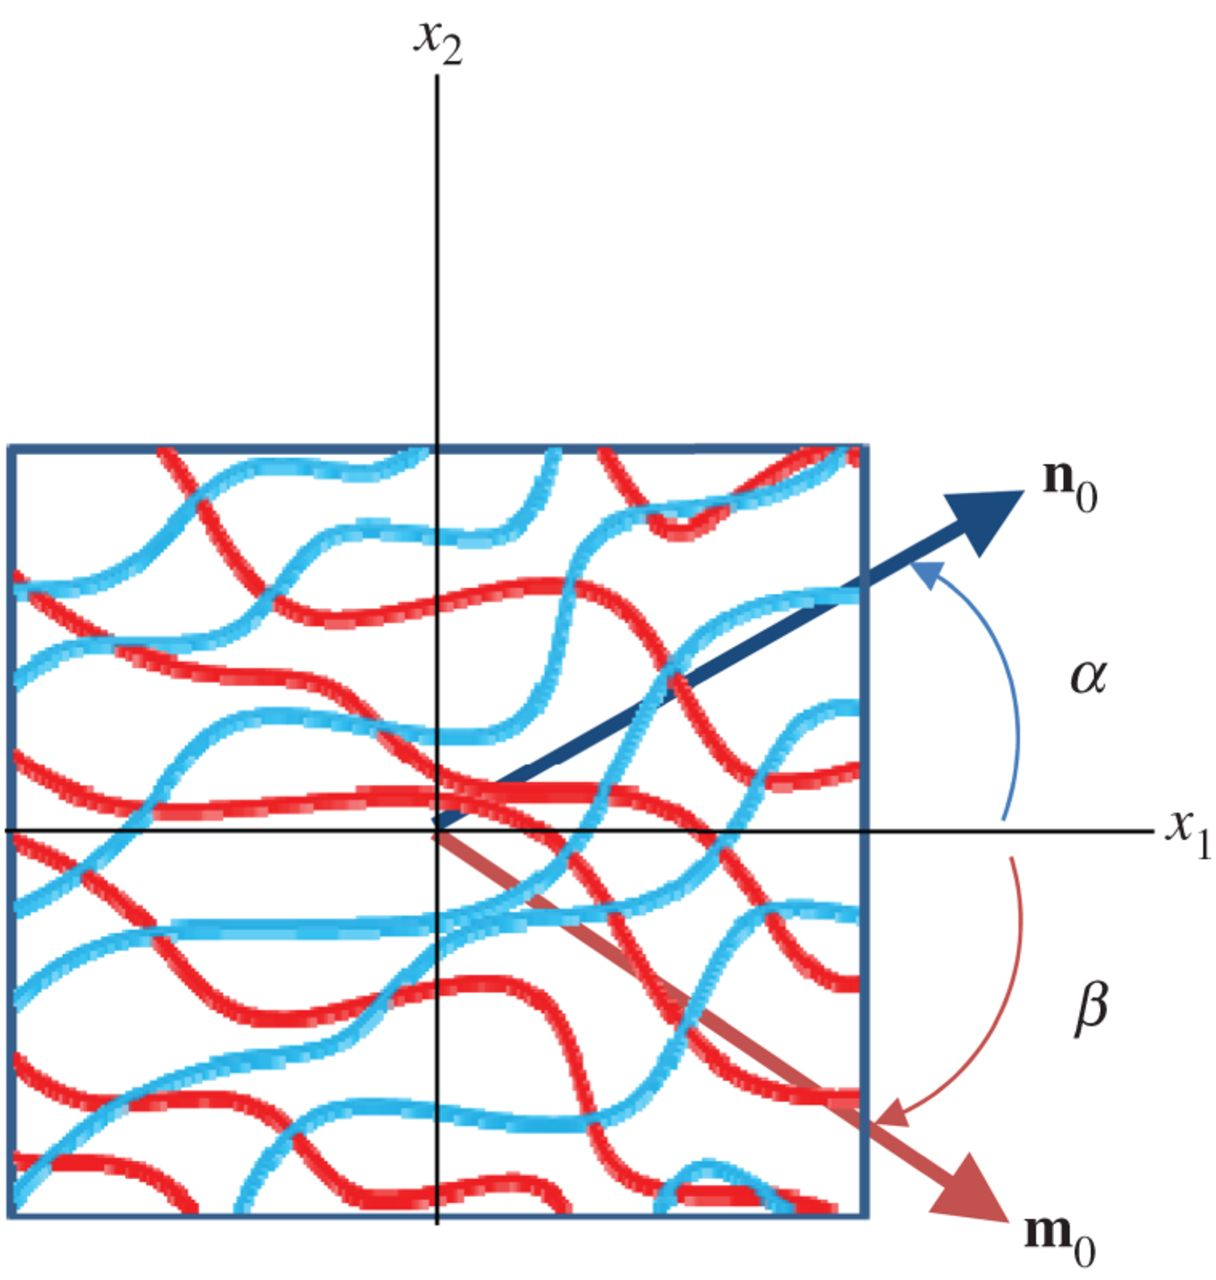
\includegraphics[width=\textwidth]{Images/chapter3/F7large.jpg}
\caption{A schematic of two collagen fibre ensembles with respective orientations $\alpha$ and $\beta$ (not restricted to be symmetric about the $X_1$-axis) with associated orientation vector $\mathbf{n}_0$ and $\mathbf{m}_0$ in the reference configuration.}
\label{c3:fig:7}
\end{figure}
%%%%%%%%%%%%%%%%%%%%	 end FIGURE 	%%%%%%%%%%%%%%%%%%%%
    
    
    To best capture these phenomena, we do not use $I_8$ directly but rather the following forms. The results for the ensemble stress suggest that the interaction terms are exponential in character (figure \ref{c3:fig:8}). Thus, for the extensional intra-ensemble effects we use
        %-------------------	begin EQUATION 	-------------------%
        \begin{equation}\label{c3:eqn:410}
        \begin{aligned}
        \Psi_\mathrm{int}^e(\mathbf{C}) = \frac{c_0}{4}\int_\theta\Gamma(\theta)\left[e^{c_1(\lambda-1)^2} - 1\right]\dif \theta
        \end{aligned}
        \end{equation}
        %-------------------	 end EQUATION 	-------------------%
    where $\lambda = \sqrt{\mathbf{n}_0\cdot\mathbf{C}\mathbf{n}_0} = \sqrt{I_4}$ and $c_0$, $c_1$ are constants, and the associated single ensemble stress extensional interaction is
        %-------------------	begin EQUATION 	-------------------%
        \begin{equation}\label{c3:eqn:411}
        \begin{aligned}
        \mathbf{S}_\mathrm{int}^e =& 2\dpd{\Psi(\mathbf{C})}{\mathbf{C}} = 2 \dpd{\Psi(\lambda)}{\lambda}\dpd{\lambda}{\mathbf{C}}
        = \int_\theta \Gamma(\theta)\left[\frac{c_0c_1(\lambda-1)e^{c_1(\lambda-1)^2}}{\lambda}\mathbf{n}_0\otimes\mathbf{n}_0\right]\dif \theta
        \end{aligned}
        \end{equation}
        %-------------------	 end EQUATION 	-------------------%
    Next, for the extensional inter-ensemble interactions, we use a similar form
        %-------------------	begin EQUATION 	-------------------%
        \begin{equation}\label{c3:eqn:412}
        \begin{aligned}
        \Psi_\mathrm{int}^{ee}(\mathbf{C}) = \frac{d_0}{4}\int_\alpha\int_\beta\Gamma(\alpha)\Gamma(\beta)\left[e^{d_1(\lambda_\alpha\lambda_\beta-1)^2} - 1\right]\dif \alpha \dif\beta
        \end{aligned}
        \end{equation}
        %-------------------	 end EQUATION 	-------------------%
    where $d_0$ and $d_1$ are parameters, with associated stresses
        %-------------------	begin EQUATION 	-------------------%
        \begin{equation}\label{c3:eqn:413}
        \begin{aligned}
        \mathbf{S}_\mathrm{int}^e =& \int_\alpha\int_\beta \Gamma(\alpha)\Gamma(\beta) \\
        &\times\left[d_0d_1(\lambda_\alpha\lambda_\beta-1)e^{d_1(\lambda_\alpha\lambda_\beta-1)^2}\left(\frac{\lambda_\beta}{\lambda_\alpha}\mathbf{n}_0\otimes\mathbf{n}_0 + \frac{\lambda_\alpha}{\lambda_\beta}\mathbf{m}_0\otimes\mathbf{m}_0\right)\right]\dif\alpha\dif\beta
        \end{aligned}
        \end{equation}
        %-------------------	 end EQUATION 	-------------------%


%%%%%%%%%%%%%%%%%%%%	begin FIGURE 	%%%%%%%%%%%%%%%%%%%%
\begin{figure}
\centering
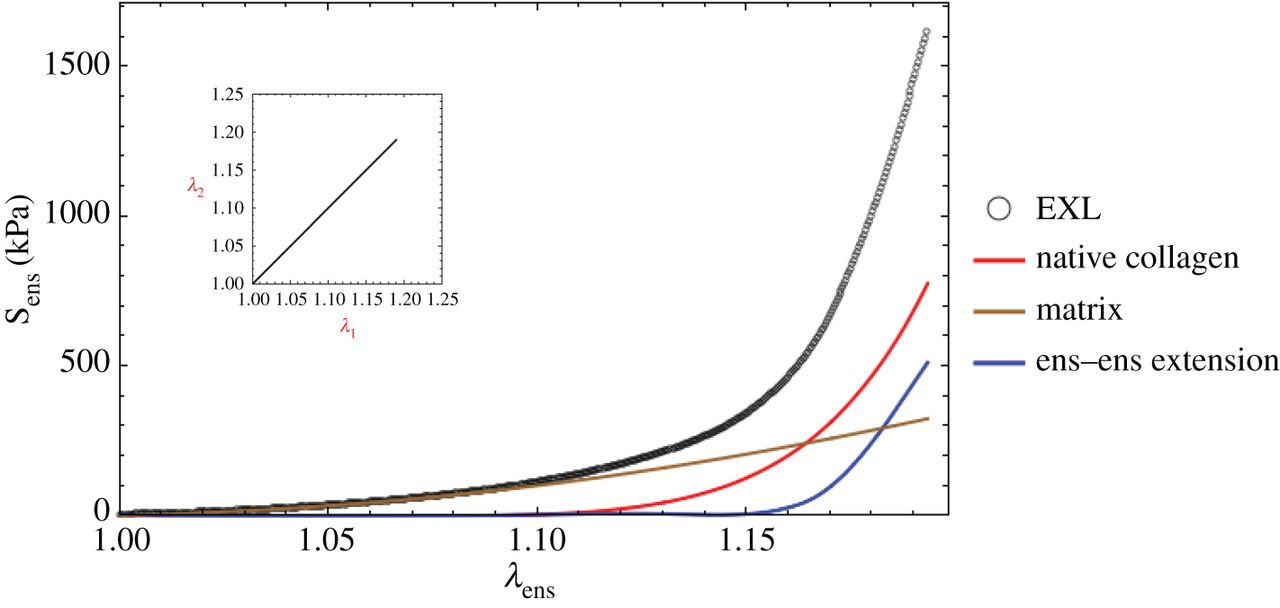
\includegraphics[width=\textwidth]{Images/chapter3/F8large.jpg}
\caption{Representative final model results (equation \ref{c3:eqn:53}) for a single fibre-ensemble stress–strain (in $S_\mathrm{ens}-\lambda_\mathrm{ens}$) response for EXL treated bovine pericardium. All model components contributed signficantly to the total stress. Surprisingly, while the collagen phase produced the greatest contribution, the interaction term was of comparable magnitude. }
\label{c3:fig:8}
\end{figure}
%%%%%%%%%%%%%%%%%%%%	 end FIGURE 	%%%%%%%%%%%%%%%%%%%%
    
    Note that the exponential term was set to zero if $\lambda_\alpha\lambda\beta<1$ In this approach, we integrate over all ensembles, weighted by their respective orientation distribution functions, to obtain the total contribution.
    
    
    Next, we developed a rotational pseudo-invariant defined as the change in the cosine between the two ensemble fibre directions, which is simply
        %-------------------	begin EQUATION 	-------------------%
        \begin{equation}\label{c3:eqn:414}
        \begin{aligned}
        I_\mathrm{int}^r(\alpha,\beta) = \frac{I_8}{\lambda_\alpha\lambda\beta} - \mathbf{n}_0\cdot\mathbf{m}_0 = \cos{\theta}-\cos{\theta_0}\approx \Delta\theta.
        \end{aligned}
        \end{equation}
        %-------------------	 end EQUATION 	-------------------%
    Using $\Psi_\mathrm{int}^r(\mathbf{C}) = \frac{\eta^r}{4}(I_\mathrm{int}^r)^2$ it can be shown that for planar distributed fibre ensembles the stress tensor is
        %-------------------	begin EQUATION 	-------------------%
        \begin{equation}\label{c3:eqn:415}
        \begin{aligned}
        \mathbf{S}_\mathrm{int}^r =& \eta^r \int_\alpha\int_\beta \Gamma(\alpha)\Gamma(\beta) \frac{I_\mathrm{int}^r(\alpha,\beta)}{\lambda_\alpha\lambda_\beta}  \\
        &\left[\left(\mathbf{m}_0\otimes\mathbf{n}_0 + \mathbf{n}_0\otimes\mathbf{m}_0\right)
        - I_8
        \left(\frac{\mathbf{n}_0\otimes\mathbf{n}_0}{\lambda_\alpha^2} + \frac{\mathbf{m}_0\otimes\mathbf{m}_0}{\lambda_\beta^2}\right)\right]\dif\alpha\dif\beta
        \end{aligned}
        \end{equation}
        %-------------------	 end EQUATION 	-------------------%
    Combining equations \ref{c3:eqn:47}\ref{c3:eqn:48}\ref{c3:eqn:411}\ref{c3:eqn:413}\ref{c3:eqn:415}, we obtain the final form of the full model stress as
        %-------------------	begin EQUATION 	-------------------%
        \begin{equation}\label{c3:eqn:416}
        \begin{aligned}
        \mathbf{S} =& \phi_c\mathbf{S}_c(\eta_c, \mu_\Gamma, \sigma_\Gamma, \mu_0, \sigma_0) + (1-\phi_c)\mathbf{S}_m(\mu_a, \mu_b, a, b) \\
        &+ \phi_c[\mathbf{S}_\mathrm{int}^e(c_0,c_1) + \mathbf{S}_\mathrm{int}^{ee}(d_0,d_1) + \mathbf{S}_\mathrm{int}^r(\eta^r)] - p\mathbf{C}^{-1}
        \end{aligned}
        \end{equation}
        %-------------------	 end EQUATION 	-------------------%
    
        
        
        

%---    Model simplifications and parameter estimation
\section{Model simplifications and parameter estimation}

\subsection{Final form}

    While in principle equation \ref{c3:eqn:416} can be implemented within a robust parameter estimation procedure, simplifications are clearly in order given its complexity (14 parameters). We first consider an equi-biaxial test wherein all fibre rotations are zero, so that $I_\mathrm{int}^r = 0$ The total interaction stress is thus given by just the following extensional contributions:
        %-------------------	begin EQUATION 	-------------------%
        \begin{equation}\label{c3:eqn:51}
        \begin{aligned}
        \mathbf{S}_\mathrm{int} =&\int_\theta \Gamma(\theta)\left[\frac{c_0c_1(\lambda-1)e^{c_1(\lambda-1)^2}}{\lambda}\mathbf{n}_0\otimes\mathbf{n}_0\right]\dif \theta  \\
        &+ \int_\alpha\int_\beta \Gamma(\alpha)\Gamma(\beta)\left[d_0d_1(\lambda^2-1)e^{d_1(\lambda^2-1)^2}\left(\mathbf{n}_0\otimes\mathbf{n}_0 + \mathbf{m}_0\otimes\mathbf{m}_0\right)\right]\dif\alpha\dif\beta
        \end{aligned}
        \end{equation}
        %-------------------	 end EQUATION 	-------------------%
    In practice, we found that while the intra-ensemble form (first r.h.s. term) was used alone it was able to capture the equi-biaxial strain behaviour (figure \ref{c3:fig:5}), it was unable to capture the response from all test protocols. Moreover, given the similarity in form, the two components on the r.h.s. of equation (5.1) can capture similar responses. We thus chose to ignore the intra-ensemble stress contribution $\mathbf{S}_\mathrm{int}^e(c_0,c_1)$ removing two parameters. Next, while it is intuitive that fibre-ensemble rotations produce important contributions to the total tissue stress, closer analysis of equation \ref{c3:eqn:415} indicated that it will produce compressive stresses in the direction of lesser stretch. These characteristics were not consistent with any of the observed experimental data. Even when choosing various forms of $\Psi_\mathrm{int}^r$ we could not match the experimentally observed responses. Interestingly, only the $S_\mathrm{int}^{ee}$ contribution of equation \ref{c3:eqn:416} was found to model the interaction stresses well.
    
    Thus, we are left with the following interaction stresses:
        %-------------------	begin EQUATION 	-------------------%
        \begin{equation}\label{c3:eqn:52}
        \begin{aligned}
        \mathbf{S}_\mathrm{int}^e =& \int_\alpha\int_\beta \Gamma(\alpha)\Gamma(\beta) \\
        &\times\left[d_0d_1(\lambda_\alpha\lambda_\beta-1)e^{d_1(\lambda_\alpha\lambda_\beta-1)^2}\left(\frac{\lambda_\beta}{\lambda_\alpha}\mathbf{n}_0\otimes\mathbf{n}_0 + \frac{\lambda_\alpha}{\lambda_\beta}\mathbf{m}_0\otimes\mathbf{m}_0\right)\right]\dif\alpha\dif\beta
        \end{aligned}
        \end{equation}
        %-------------------	 end EQUATION 	-------------------%
    leading to the following final form of the constitutive model:
        %-------------------	begin EQUATION 	-------------------%
        \begin{equation}\label{c3:eqn:53}
        \begin{aligned}
        \mathbf{S} =& \mathbf{S}_c + \mathbf{S}_{int} + \mathbf{S}_m  \\
        =& \phi_c\frac{\eta_c}{\prescript{t}{1}{\lambda}} \int_{\theta_1} \Gamma_1(\mu_\Gamma, \sigma_\Gamma,\theta_1))
        \frac{D_1(x)}{x}\left(\frac{\prescript{1}{0}{\lambda}}{x} - 1\right)\mathbf{n}_1\otimes\mathbf{n}_1 \dif x \dif \theta \\
        +& \phi_c\int_\alpha\int_\beta \Gamma(\alpha)\Gamma(\beta) d_0d_1(\lambda_\alpha\lambda_\beta-1)e^{d_1(\lambda_\alpha\lambda_\beta-1)^2}\left(\frac{\lambda_\beta}{\lambda_\alpha}\mathbf{n}_0\otimes\mathbf{n}_0 + \frac{\lambda_\alpha}{\lambda_\beta}\mathbf{m}_0\otimes\mathbf{m}_0\right)\dif\alpha\dif\beta    \\
        +&(1-\phi_c) \left(\mu_a(I_1 - 3)^{a-1} + \mu_b(I_1 - 3)^{b-1}\right)(\mathbf{I} - C_{33}\mathbf{C}^{-1}), \\
        \end{aligned}
        \end{equation}
        %-------------------	 end EQUATION 	-------------------%
        It is understood that $\mathbf{n}_0$ and $\mathbf{m}_0$ are referred to $\beta_1$ and that we merged the Lagrange multiplier with the matrix by assuming a planar tissue to simplify the formulation. This final model has 11 independent fitted parameters \{$\eta_c$, $\mu_\Gamma$, $\sigma_\Gamma$, $\mu_0$, $\sigma_0$, $d_0$, $d_1$, $\mu_a$, $\mu_b$, $a$, $b$\} and three directly determined parameters $\phi_c, \prescript{}{0}{\lambda}_{lb}, \prescript{}{0}{\lambda}_{ub}$ all with a physical meaning.
        
        
        
        
\subsection{Parameter estimation procedures}

    While at first glance this appears to be a major nonlinear optimization undertaking with all the usual pitfalls, we can use the following sequence to make actual parameter estimation quite tractable:
        \begin{enumerate}
            \item From the native tissue mechanical data, predict the collagen phase parameters $\{\eta_c, \mu_\Gamma, \sigma_\Gamma, \mu_0, \sigma_0\}$ using standard procedures \cite{fata_insights_2014,zhang_meso_2016}.
            \item From the pre-transition collagen recruitment portion of all of the EXL tissue mechanical data, determine the matrix parameters $\{\mu_a, \mu_b, a, b\}$.
            \item Taking the collagen and matrix responses, determine the interaction stress responses for all test protocols using $\mathbf{S}_\mathrm{int} = \mathbf{S} - \frac{1}{\phi_c}\left(\phi_c \prescript{1}{0}{S}_c + (1-\phi_c)\mathbf{S}_m\right)$
            \item Using the results of step 3, determine the final two parameters ($d_0$ and $d_1$) by fitting equation \ref{c3:eqn:53} but only allowing them to vary while keeping the other terms to their above-fitted values.
        \end{enumerate}
    We found that this basic sequence ensured a robust parameter is obtained, because the entire model is never fitted at once. Moreover, this approach allowed us to separate the contributions to the stress of each of these mechanisms. As in our previous studies \cite{fata_insights_2014,zhang_meso_2016}, we employed the genetic based Differential Evolution algorithm in Mathematica to perform the optimization. All parameter estimation was performed using a custom program written in Mathematica (Wolfram Research Corp.).

        
        

%---    primary results
\section{Primary results}
    
    From the five specimens used, the model was able to successfully fit all data quite well (total fit $r^2 > 0.97$). Moreover, the final parameter values were quite consistent, with generally low standard errors (table 3). The mean collagen fibre modulus (approx. 279 MPa) and fibre splay (approx. $38^\circ$) were comparable to previous studies \cite{fan_simulation_2014}. Interestingly, the lower bound stretch was small (1.01 or approx. 1\% strain), 
    so it is likely that it could be set to 1 (i.e. zero strain). The native collagen fibre recruitment parameters were also consistent (table 3), and indicated a very rapid recruitment at stretch of approximately 1.18–1.2 (figure 9). This is a more complete picture of the entire fibre recruitment than in our previous work \cite{sun_finite_2005}\cite{fan_simulation_2014}, and suggests that the collagen fibres are effectively well ordered with a small deviation in crimp amplitude and wavelength.
    

\begin{table}
\centering
\caption{Equibiaxial strain testing results.}\label{c3:tab:3}
\begin{tabular}{L{.5in}R{.7in}R{0.5in}R{0.5in}R{0.6in}R{0.5in}R{0.6in}R{0.5in}}
\hline
& \multicolumn{1}{c}{\textbf{modulus}} & \multicolumn{2}{c}{\textbf{ODF}} & \multicolumn{4}{c}{\textbf{recruitment}}\\
\cline{2-8}
& $\eta_c(MPa)$ & $\mu_\Gamma({}^\circ)$ & $\sigma_\Gamma({}^\circ)$ & $\mu_0$ & $\sigma_0$ & $\prescript{}{0}{\lambda}_{lb}$
& $\prescript{}{0}{\lambda}_{ub}$\\
mean & 278.94 & 6.513 & 38.430 & 1.185 & 0.014 & 1.011 & 1.197  \\
s.e.m. & 22.38 & 1.645 & 0.922 & 0.032 & 0.001 & 0.007 & 0.035  \\
\hline
\hline
& \multicolumn{2}{c}{\textbf{Interactions}} & & \multicolumn{4}{c}{\textbf{Matrix}} \\
\cline{2-8}
& $d_0(kPa)$ & $d_1$ & & $\mu_a(kPa)$ & $a$ & $\mu_b(kPa)$ & $b$\\
mean & 1.040 & 42.267 & & 56.74 & 1.068 & 1294.38 & 1.873  \\
s.e.m. & 0.255 & 9.772 & & 10.69 & 0.004 & 340.71 & 0.007 \\
\hline
\end{tabular}
\end{table}


    One advantage of our approach is that the various contributions to the total stress can be separated (figure 8). To better reveal the present findings, it is useful to examine the effects on the individual stress components under various loading paths. Following the trends of the ensemble results (figure 9), we noted that the interactions produced substantial contributions to the total stress (figure 10). Interestingly, for $S_{11}$ the interactions actually produced the largest contributions, followed by the matrix and collagen fibres. By contrast, for $S_{22}$ the contributions were much more dependent on the particular loading path, with the collagen phase dominating when $\lambda_2>\lambda_1$. When $\lambda_1>\lambda_2$, the matrix phase dominated $S_22$. We further note here that the contribution of the matrix was much less loading path sensitive, due to its near-linear, isotropic behaviour.

%---    discussion
\section{Discussion}

\subsection{Major findings}

    This study represents the first rigorous full structural model (i.e. explicitly incorporating various features of the CFA) for cross-linked soft tissues, and also includes a specific interaction term. An important utility of this model is its ability to separate the effects of EXLs on the fibres and matrix, so that the matrix, collagen and interaction effects could be clearly identified. This was made possible, in-part, with the use of the native–EXL matched experimental dataset and a modification to the structural model so that the uncross-linked collagen fibre responses could be mapped to the EXL configuration. As in our previous study, we found that the matrix could be well modelled as an isotropic material. However, we found that a much more linear-like response was necessary. Perhaps the most novel findings of this study were that (i) the effective collagen fibre modulus was unaffected by cross-linking and (ii) the interaction term played such a large role in stress development, often dominating the response (depending on the component and loading path being considered).
    
    
    The lack of change in the effective collagen fibre modulus has been corroborated by experimental results from Gentleman et al. \cite{gentleman_mechanical_2003}. In that study, they found a modulus range of $269.7\pm11.9$ to $ 484.7\pm76.3$ for cross-linked collagen fibres in the bovine Achilles tendon, which corresponds to the same range as another study for native collagen fibres from various sources \cite{eppell_nano_2006}. Yang et al. \cite{yang_mechanical_2008}\cite{yang_micromechanical_2007} determined that for the mechanical properties of hydrated native and cross-linked type I collagen fibrils that cross-linking the collagen fibrils with a water-soluble carbodiimide did not significantly affect the bending modulus. The work by Shen et al. \cite{shen_stress_2008} noted a modulus of $0.86\pm0.45$ GPa (range, 0.36–1.60 GPa; n = 13), in reasonable agreement with our results. Further, six of the 13 fibrils showed linear behaviour. At the tissue level, our findings are also consistent with the findings of Lee et al. \cite{lee_bovine_1989I}\cite{lee_bovine_1989II}\cite{lee_bovine_1989III}, who found no change in MTM in cross-linked pericardial tissues as in our study (table \ref{c3:tab:2}). It is interesting to note that, when using the native tissue fibre-ensemble model (equation \ref{c3:eqn:44}) on both the native and cross-linked data (figure 5), one can increase the fibre modulus determined from the native state to match the post-EXL data (figure 11a). However, this will induce a parallel increase in the MTM of approximately 75\% (figure 11b), which is inconsistent with the experimental findings (table \ref{c3:tab:2}). This is the case even when compensating for the effects of tissue contraction. This simple simulation lends support to the collagen modulus results (figure 5c).
    
    
    Our model results suggest that the major effect of EXL formation was not the formation of a mechanically substantial matrix or stiffening of the collagen fibres, but rather a dramatically enhanced bonding both within and between fibre ensembles. Note that our specific interaction term (equation \ref{c3:eqn:413}) captured the effects of both individual ensemble stretch and relative stretching between ensembles. This is consistent with what is known about GLUT bond formations (figure 1a) \cite{nimni_chemically_1987}\cite{cheung_mechanism_1985}\cite{cheung_presence_1983}\cite{cheung_mechanism_1982}\cite{cheung_mechanism_1982II}. Yet, we found that relative rotations between fibre ensembles as modelled by equation \ref{c3:eqn:415} could not capture the observed responses. The underlying structural mechanisms for this behaviour remain largely uncharacterized. One possibility is that the protein core of the proteoglycans that bind collagen fibrils become strongly cross-linked and are thus substantially stiffened, acting to more cohesively bind the collagen fibres. This is supported by findings of Liao \& Vesely \cite{liao_relationship_2004}, who observed substantial deformations of proteoglycans in mitral valve chordae under stretch. Moreover, the present model suggests that such mechanisms are strongly associated with fibre-ensemble orientation distributions. While not the final word, our results suggest that EXLs produce a stiffening effect via an isotropic matrix, with the interaction effects being the dominant effect.
    
    


\subsection{Modelling approach}

    The present approach was a direct extension of the stochastic, tissue-level meso-structural models first pioneered by Lanir \cite{lanir_constitutive_1983} and used in various applications and extensions by our group \cite{sacks_incorporation_2003}\cite{fata_insights_2014}\cite{zhang_meso_2016}. By meso-scale, we refer to the fibre-ensemble scale, which is fibre features down to approximately 100 $\mu$m. Moreover, recent evidence has demonstrated that the underlying affine kinematic assumption is valid \cite{fata_insights_2014}\cite{fan_simulation_2014}, so that the strain energy of each fibre ensemble can be kinematically connected with the macroscopic strain tensor. We took the approach to develop a more general model first, then show what components could be modified or removed entirely. Given the lack of knowledge and modelling efforts in this area, we felt this was appropriate and helped to illustrate what underlying mechanisms should be incorporated. We also considered a more extensive approach based on elastica-based theory for sinusoidal fibres based on \cite{garikipati_elastica_2008} under the assumption that EXL formation dramatically increased the fibre modulus, which ultimately proved to be unnecessary. An inter-fibre sliding model was also developed based on the relative sliding between fibres due to differences between their respective slack lengths, and used as a means to model the intra-ensemble EXL effects. However, this approach was found to be unable to capture the individual fibre-ensemble responses, suggesting that relative sliding between fibres at the ensemble level was not a major mechanism. A final question that may impact physical plausibility of the current model is convexity and physical plausibility. Lanir \cite{lanir_plausibility_1994} demonstrated that the native tissue structural model is compatible with a physically plausible response. Based on both this and the experimental observations, we focused on monotonically increasing functions of strain for all model terms to ensure physical plausibility and that convexity was maintained.
    



\subsection{Limitations and future directions}

    The current model is limited in the fact that it is quasi-static and does not account for permanent set phenomena we have observed \cite{sun_response_2004}. The homogenization method used in section \ref{c3:sec:3} is fairly standard and has been used by others and the author for some time (e.g. \cite{sacks_incorporation_2003}\cite{fata_insights_2014}\cite{fan_simulation_2014}). We have observed that for soft tissues, whose composition is dominated by a dense network of distinct fibres, especially collagen type I and elastin, these structures can be mechanically treated as fibre ensembles; that is, groups of fibres with a common orientation. The scale of the representative volume element is about 100 $\mu$m, which is sufficient to capture the salient mechanical features of the fibre ensemble. We emphasize that this is not meant to be a universal model of all types of soft tissue structures, which are very diverse for a single theoretical treatment. Rather, we focus on a sufficiently generalized approach for exogenously cross-linked dense collagenous tissues, such as pericardium, heart valves and sclera. These structures fit our approach well and also have important biomedical therapeutic applications.


    A complete understanding of the current phenomena must be based on well-characterized micro-scale events. For example, Kojic et al. \cite{kojic_numerical_1998} developed a model for fibre–fibre kinetics that uses Coulomb friction, which results in a simple and robust approach for tissue simulations. However, our knowledge of even native tissues at the micro-level remains limited. The situation remains more complicated by the fact that our knowledge of the interrelationships between the physical chemistry of EXLs and the macro-scale mechanics of collagenous tissues remains limited at the present time for more sophisticated models to be reliably attempted. To date, no material model is able to fully account for such complex observed microstructural and biological behaviour. The next steps include incorporation of the permanent set effect commonly observed in cross-linked tissues into the present model, and exploration of how alternative cross-linking methods affect macro-scale tissue behaviours.

%%%%%%%%%%%%%%%%%%%%%%%%%%%%%%%%%%%%%%%%%%%%%%%%%%%%%%%%%%%%%
%%  nomenclature											%
%%%%%%%%%%%%%%%%%%%%%%%%%%%%%%%%%%%%%%%%%%%%%%%%%%%%%%%%%%%%%
\section*{Nomenclature} \label{c3:sec:nomenclature}
\begin{mynom}
{int}\>\tabfill{Interaction term} \\
{c}\>\tabfill{Collagen} \\
{m}\>\tabfill{Matrix} \\
{EB}\>\tabfill{Equibiaxial} \\
{ODF}\>\tabfill{Orientation distribution functio z} \\
{$\mathbf{F}$}\>\tabfill{Deformation gradient tensor} \\
{$\mathbf{E}$}\>\tabfill{Green Lagrange strain} \\
{$\mathbf{P}$}\>\tabfill{First Piola Kirchhoff stress tensor} \\
{$\mathbf{S}$}\>\tabfill{Second Piola Kirchhoff tensor} \\
{$\mathbf{C}$}\>\tabfill{Right Cauchy-Green strain tensor} \\
{$\mathbf{m}_0$,$\mathbf{n}_0$}\>\tabfill{fibre-ensemble orientation vectors} \\
{$_ens$}\>\tabfill{ensemble} \\
{$\lambda$}\>\tabfill{Stretch} \\
{$\lambda_s$}\>\tabfill{The slack stretch, the stretch needed to straighten the collagen fiber crimp} \\
{$\lambda_t$}\>\tabfill{The true stretch after the collagen fibers are straightened} \\
{$E_s$}\>\tabfill{The slack strain} \\
{$\Psi$}\>\tabfill{The strain energy} \\
{$\phi$}\>\>\tabfill{The mass fractions} \\
{$D$}\>\tabfill{Distribution of slack strains for fibre recruitment} \\
{$\Gamma$}\>\tabfill{Fiber orientation distribution function} \\
{$\eta$}\>\tabfill{modulus, subscript for elastin collagen and matrix} \\
{$\mu_\theta$}\>\tabfill{mean circumferential orientation} \\
{$\sigma$}\>\tabfill{standard deviation of the fibre splay} \\
{$\mu_r$}\>\tabfill{mean of the recruitment distribution} \\
{$\sigma_r$}\>\tabfill{standard deviation of the recruitment distribution} \\
{$\lambda_{lb}$}\>\tabfill{lower bound of the recruitment distribution} \\
{$\lambda_{ub}$}\>\tabfill{upper bound of the recruitment distribution} \\
{$c_0$, $c_1$}\>\tabfill{exponent for intra-fibre-ensemble interaction terms} \\
{$d_0$, $d_1$}\>\tabfill{exponent for inter-fibre-ensemble interaction terms}
\end{mynom}

%---    Bioliography
\bibliographystyle{plainnat}
\bibliography{phd}